\documentclass[12pt,a4paper]{extarticle}
\usepackage[left=25mm,right=20mm,top=20mm,bottom=20mm]{geometry}
\usepackage{fontspec}
\IfFontExistsTF{Times New Roman}{\setmainfont{Times New Roman}}{\setmainfont{Liberation Serif}}
\setmonofont{DejaVu Sans Mono}[Scale=0.8]
\usepackage{polyglossia}
\setdefaultlanguage{russian}
\setotherlanguage{english}
\usepackage{amsmath,amssymb,graphicx,booktabs,tabularx,array}
\usepackage{setspace,caption,float,enumitem,titlesec}
\usepackage[unicode,hidelinks]{hyperref}
\hypersetup{pdfauthor={Шешуков Евгений Игоревич},pdflang={ru-RU}}
\setstretch{1.15}
\setlength{\parindent}{1.25cm}
\setlength{\parskip}{3pt}
\setlength{\emergencystretch}{2em}
\setlength{\tabcolsep}{5pt}
\setlength{\intextsep}{8pt}
\renewcommand{\arraystretch}{1.18}
\captionsetup{font=small,labelsep=colon,justification=centering}
\setlist{nosep,topsep=5pt,leftmargin=1.4cm}
\titleformat{\section}{\large\bfseries}{\thesection.}{0.5em}{}
\titleformat{\subsection}{\normalsize\bfseries}{\thesubsection.}{0.5em}{}
\titlespacing*{\section}{0pt}{12pt}{7pt}
\titlespacing*{\subsection}{0pt}{9pt}{4pt}
\setlength{\abovedisplayskip}{7pt}
\setlength{\belowdisplayskip}{7pt}
\widowpenalty=10000
\clubpenalty=10000
\raggedbottom
\newcommand{\code}[1]{\texttt{\small #1}}
\newcommand{\reporttitle}[2]{%
\hypersetup{pdftitle={Лабораторная работа №#1. #2}}
\begin{titlepage}
\begin{center}
{\bfseries БЕЛОРУССКИЙ ГОСУДАРСТВЕННЫЙ УНИВЕРСИТЕТ\par}
\vspace{4mm}
{\bfseries ФАКУЛЬТЕТ ПРИКЛАДНОЙ МАТЕМАТИКИ\par И ИНФОРМАТИКИ\par}
\vspace{4mm}
Кафедра компьютерных технологий и систем
\vspace{34mm}

{\Large\bfseries ОТЧЁТ ПО ЛАБОРАТОРНОЙ\par РАБОТЕ №#1\par}
\vspace{7mm}
{\Large\bfseries «#2»\par}
\vspace{7mm}
Дисциплина: Компьютерная графика\par
\vspace{3mm}
Вариант 13
\end{center}
\vspace{24mm}
\hfill\begin{minipage}{0.57\textwidth}
\textbf{Выполнил:}\par
студент 3 курса 2 группы\par
Шешуков Евгений Игоревич\par
\vspace{6mm}
\textbf{Преподаватель:}\par
Каркоцкий Александр Геннадьевич
\end{minipage}
\vfill
\begin{center}Минск, 2026\end{center}
\end{titlepage}
\setcounter{page}{2}}

\newcommand{\comparisonlabels}[3]{%
\makebox[0.32\textwidth]{\small #1}\hfill
\makebox[0.32\textwidth]{\small #2}\hfill
\makebox[0.32\textwidth]{\small #3}\par\vspace{2mm}}
\newcommand{\comparisonrow}[3]{%
\setlength{\fboxsep}{0pt}\setlength{\fboxrule}{0.3pt}%
\fbox{\includegraphics[width=0.318\textwidth]{#1}}\hfill
\fbox{\includegraphics[width=0.318\textwidth]{#2}}\hfill
\fbox{\includegraphics[width=0.318\textwidth]{#3}}}
\begin{document}
\reporttitle{2}{Основы обработки цифровых изображений}

\section{Цель и задание}
Реализовать методы обработки изображений, сравнить их действие на подходящих примерах и объяснить различия результатов.

Номер в списке группы --- 13. В таблице задания ему соответствуют третья строка и третий столбец:
\begin{enumerate}
\item локальная пороговая обработка: два метода на выбор;
\item высокочастотные фильтры для увеличения резкости.
\end{enumerate}
Для первой части выбраны методы Ниблэка и Сауволы. Во второй части реализованы фильтр на основе лапласиана и нерезкое маскирование. Приложение имеет графический интерфейс, позволяет менять параметры и сохранять результаты в исходном разрешении.

\section{Представление и подготовка данных}
Исходное изображение хранится как массив RGB с целыми компонентами от 0 до 255. При чтении учитывается ориентация EXIF, а прозрачные пиксели накладываются на белый фон. Для бинаризации вычисляется полутоновое изображение:
\begin{equation}
 I(x,y)=\operatorname{round}\bigl(0.299R(x,y)+0.587G(x,y)+0.114B(x,y)\bigr).
\end{equation}
Фильтры резкости применяются отдельно к каждому каналу RGB.

В набор включены четыре синтетических изображения размером $720\times480$ пикселей и два эталона. Скрипт \code{make\_samples.py} создаёт:
\begin{itemize}
\item текст на фоне с плавной тенью и гауссовым шумом со стандартным отклонением 3 уровня яркости;
\item бледный текст: фон 220, непрозрачные штрихи 198, разница 22 уровня;
\item цветные фигуры, текст и тонкие линии с гауссовым размытием радиуса 1.5 пикселя;
\item ту же сцену с гауссовым шумом со стандартным отклонением 9 уровней в каждом RGB-канале.
\end{itemize}
Эталоны --- маска текста и исходная сцена без искажений. Генератор случайных чисел использует фиксированное начальное значение 13. Для эталонной маски текстом считается покрытие штриха не менее $0.5$. Эти данные позволяют проверить оба возможных исхода сравнения пороговых методов, а также пользу и ограничения повышения резкости.

\clearpage
\section{Локальная пороговая обработка}
Для каждого пикселя рассматривается квадратное окно $W_{xy}$ нечётного размера $w\times w$. Среднее и стандартное отклонение в окне равны
\begin{equation}
 m=\frac{1}{w^2}\sum_{(u,v)\in W_{xy}}I(u,v),\qquad
 s=\sqrt{\max\left(\frac{1}{w^2}\sum_{(u,v)\in W_{xy}}I(u,v)^2-m^2,0\right)}.
\end{equation}
Ограничение снизу нулём устраняет небольшую отрицательную погрешность дисперсии. За границами изображения повторяется ближайший крайний пиксель.

\subsection{Методы Ниблэка и Сауволы}
В использованной записи порог Ниблэка имеет вид
\begin{equation}
 T_N(x,y)=m(x,y)-k_Ns(x,y).
\end{equation}
При $k_N=0.2$ порог находится немного ниже локального среднего. При записи формулы с плюсом этому соответствует коэффициент $-0.2$.

Для метода Сауволы используется
\begin{equation}
 T_S(x,y)=m(x,y)\left[1+k_S\left(\frac{s(x,y)}{R}-1\right)\right],\qquad R=128.
\end{equation}
Параметры по умолчанию: $w=31$, $k_N=k_S=0.2$. В обоих случаях тёмный текст выделяется одним правилом:
\begin{equation}
 B(x,y)=\begin{cases}0,&I(x,y)<T(x,y),\\255,&I(x,y)\ge T(x,y).\end{cases}
\end{equation}
Равенство относится к фону. Поэтому однородная область, включая полностью чёрное изображение, при выбранных параметрах становится белой: локальных перепадов в ней нет.

\subsection{Расчёт и особенности реализации}
Пусть $m=220$, $s=10$ и $k_N=k_S=0.2$. Тогда $T_N=218$, а $T_S=179.4375$. Пиксель со значением 198 станет чёрным у Ниблэка и белым у Сауволы. Этот пример объясняет, почему Саувола может потерять слабый текст на светлом фоне.

Суммы яркостей и их квадратов вычисляются через интегральные изображения. Сумма в прямоугольнике получается по четырём значениям префиксной суммы. После её построения каждое окно обрабатывается за постоянное число операций; не требуется отдельно складывать все $w^2$ пикселей. Вычисления выполняются в \code{float64}.

\clearpage
\section{Повышение резкости}
Высокочастотная составляющая выделяет быстрые изменения яркости. Её добавление к исходному изображению подчёркивает границы, но одновременно может усилить шум.

\subsection{Фильтр на основе лапласиана}
Используется разностный оператор с четырьмя соседями:
\begin{equation}
 \Delta I(x,y)=I(x-1,y)+I(x+1,y)+I(x,y-1)+I(x,y+1)-4I(x,y).
\end{equation}
Результат вычисляется как $J=I-a\Delta I$. Высокочастотная добавка $-\Delta I$ соответствует ядру
\begin{equation}
 K=\begin{bmatrix}0&-1&0\\-1&4&-1\\0&-1&0\end{bmatrix}.
\end{equation}
Сумма его коэффициентов равна нулю, поэтому постоянная область не меняется. По умолчанию $a=0.6$. Если центральный пиксель равен 100, а каждый сосед --- 90, то $\Delta I=-40$ и новое значение равно $100-0.6(-40)=124$.

\subsection{Нерезкое маскирование}
Из изображения вычитается его сглаженная копия, затем разность добавляется с коэффициентом усиления:
\begin{equation}
 J=I+a(I-G_\sigma*I).
\end{equation}
По умолчанию $a=1.5$, $\sigma=1.2$. Одномерное гауссово ядро строится и нормируется по формуле
\begin{equation}
 g(t)=\frac{\exp(-t^2/(2\sigma^2))}{\sum_{j=-r}^{r}\exp(-j^2/(2\sigma^2))},
 \qquad t=-r,\ldots,r,\quad r=\lceil3\sigma\rceil.
\end{equation}
Двумерная свёртка разделяется на горизонтальную и вертикальную. На границах повторяются крайние пиксели. Промежуточные значения остаются вещественными; округление и ограничение диапазоном $[0,255]$ выполняются только при формировании результата.

При большом усилении возможны светлые и тёмные ореолы около границ, а также обрезка значений до 0 или 255. Поэтому коэффициент усиления выбирается по изображению; увеличение параметра не гарантирует улучшения результата.

\clearpage
\section{Интерфейс приложения}
В каждой вкладке рядом показаны исходное изображение и результаты двух методов. Изменения параметров применяются кнопкой «Обработать» или клавишей Enter.
\begin{figure}[H]
\centering
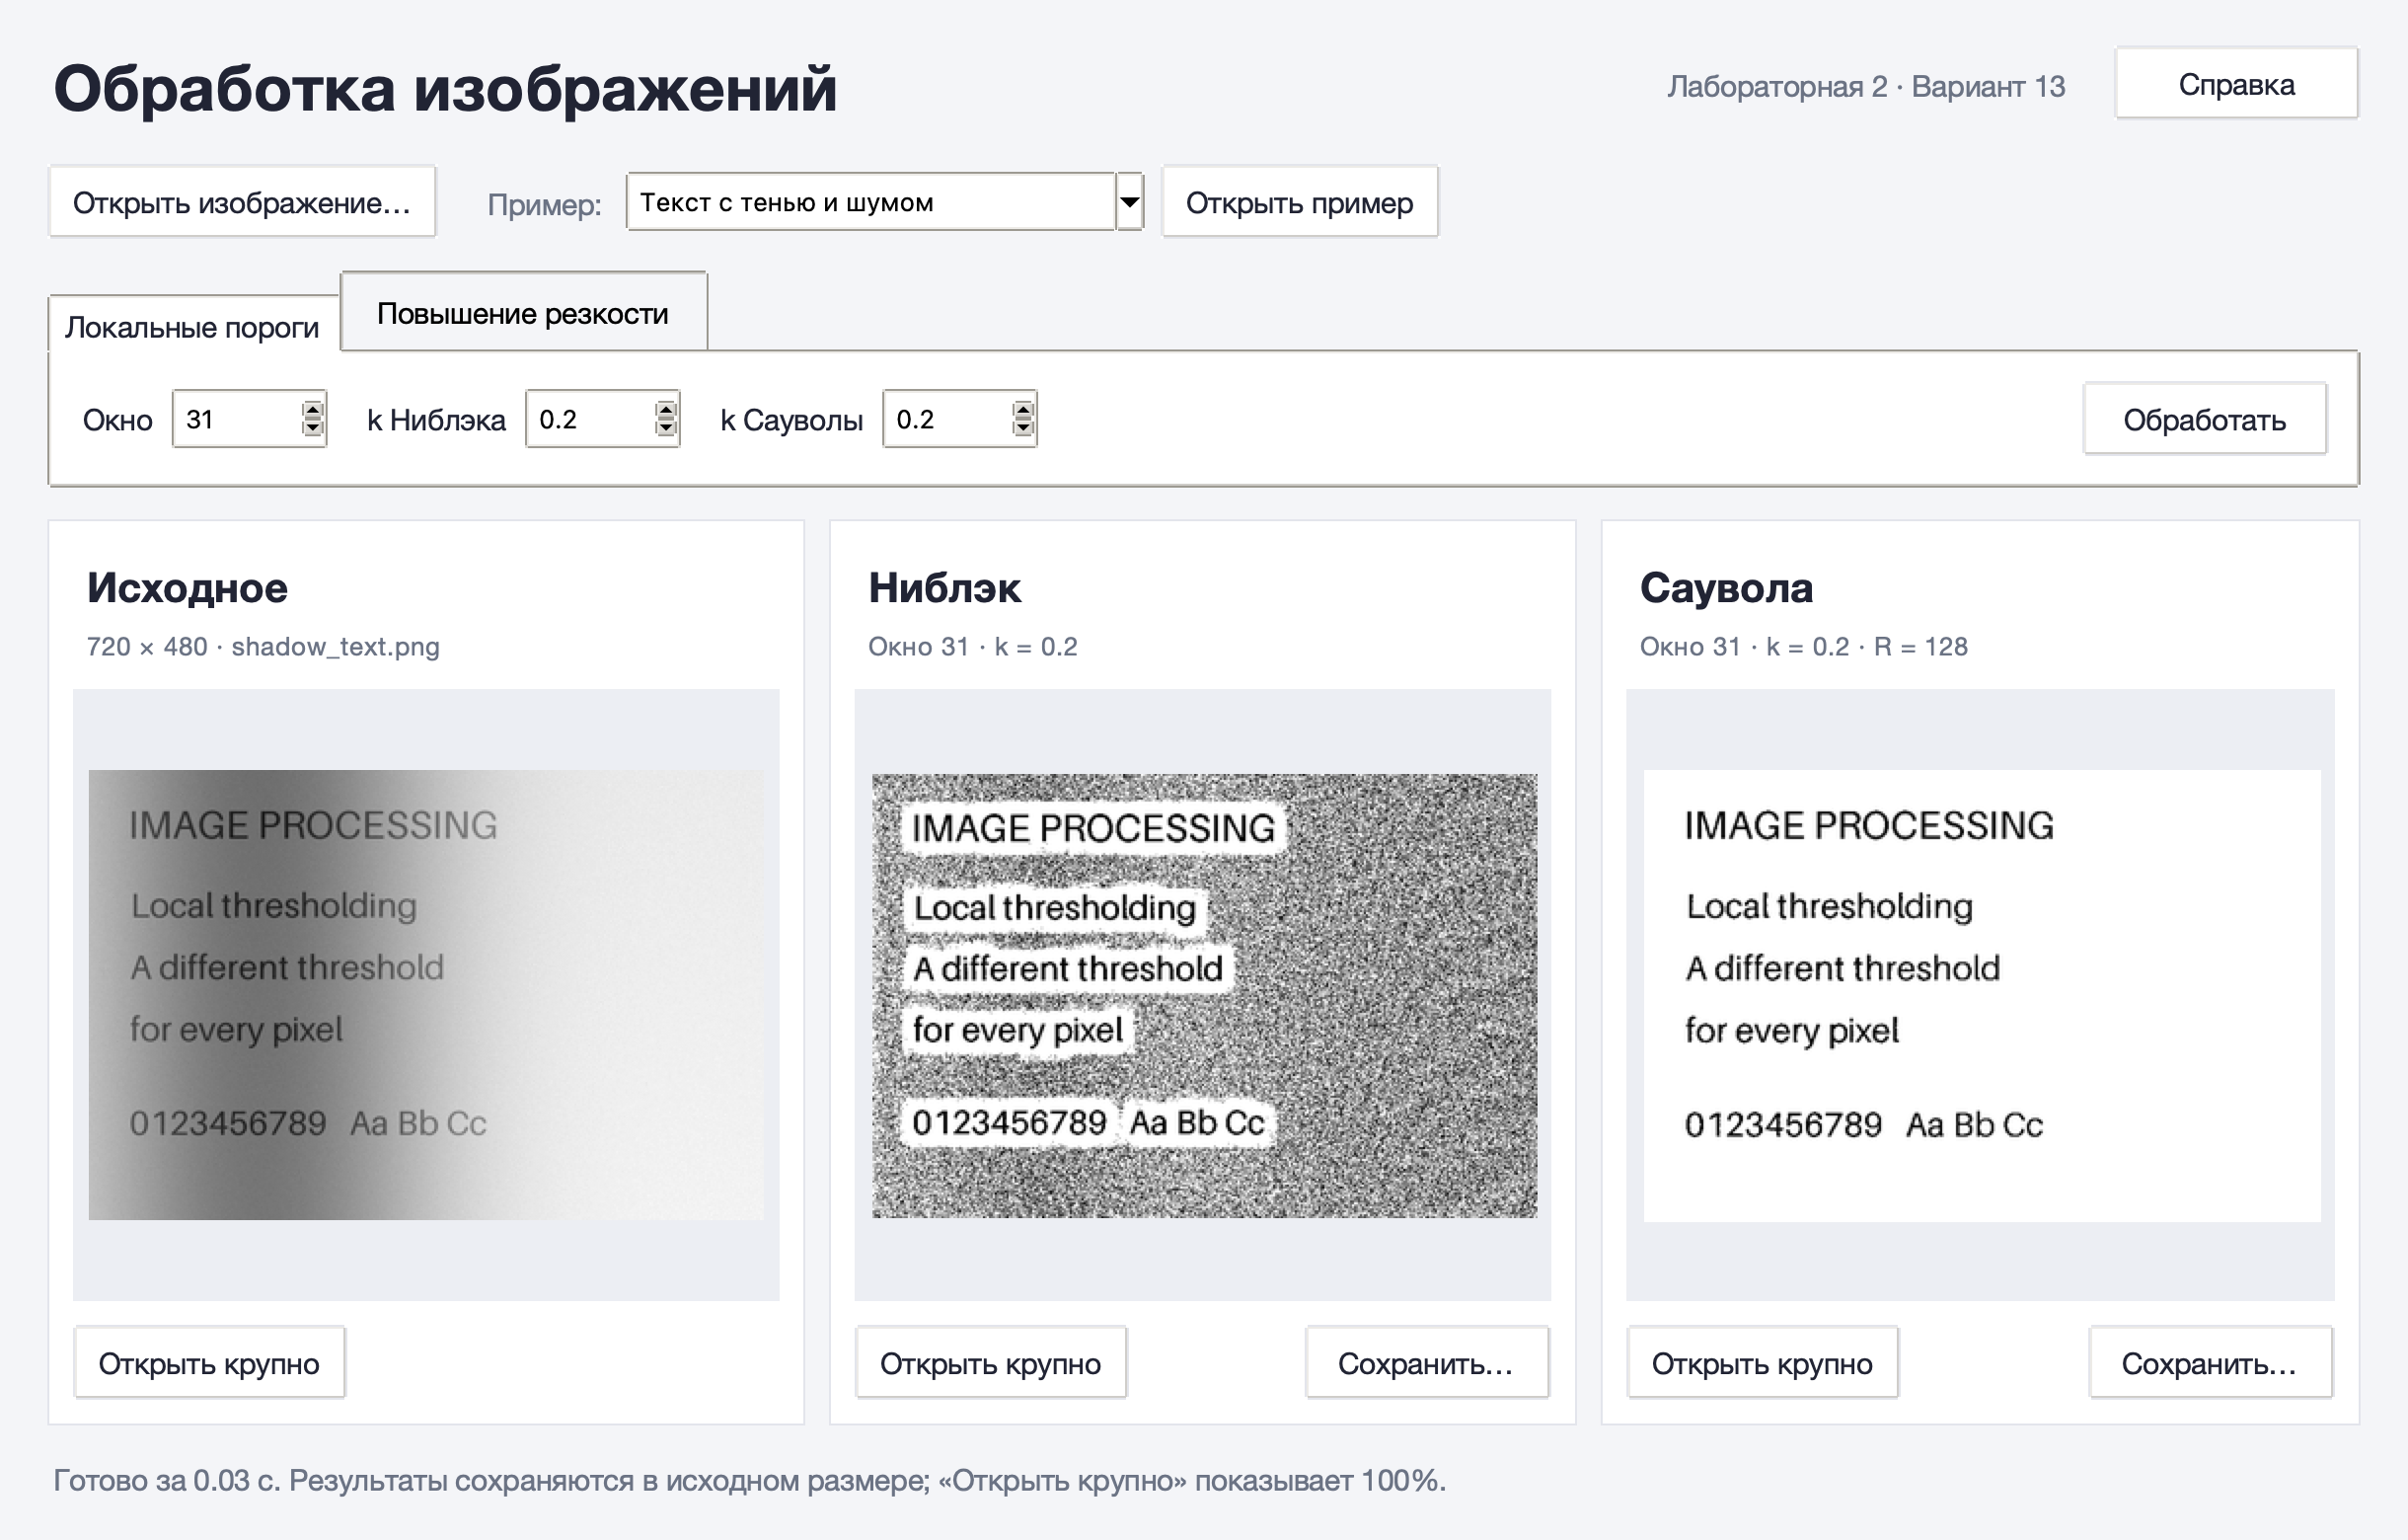
\includegraphics[width=0.92\textwidth]{../docs/thresholds.png}
\caption{Локальные пороги: сравнение Ниблэка и Сауволы}
\end{figure}
\begin{figure}[H]
\centering
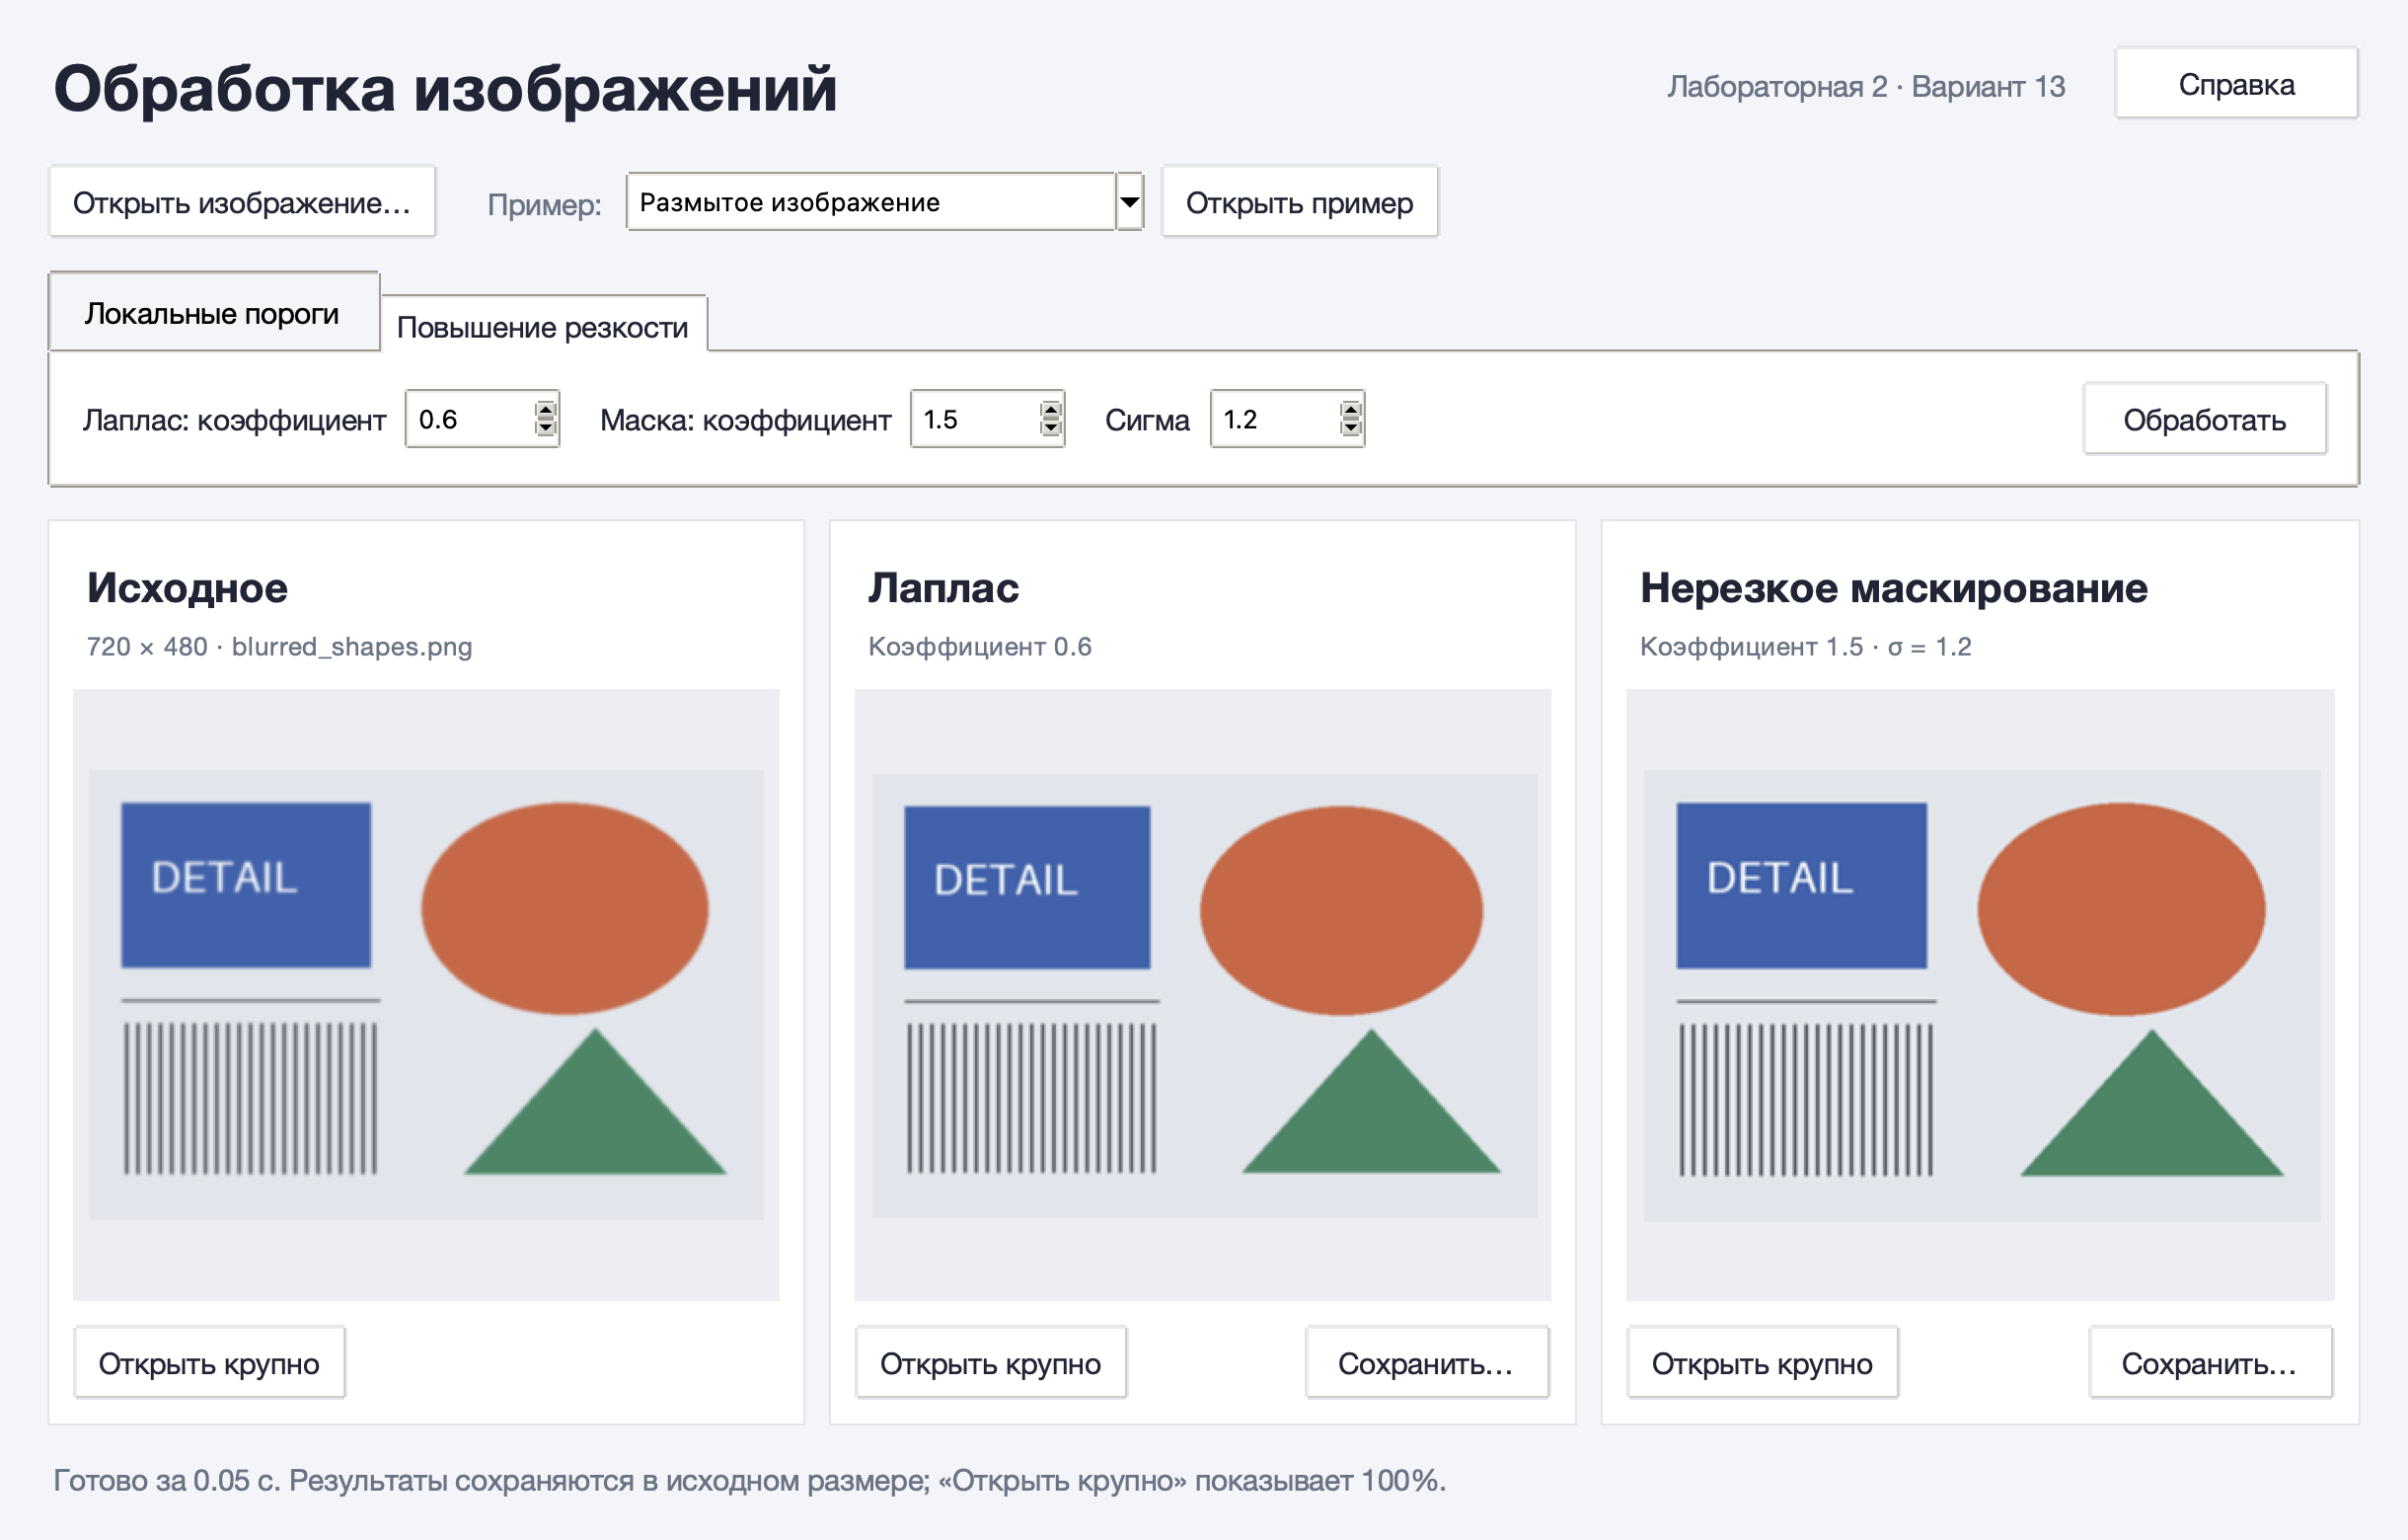
\includegraphics[width=0.92\textwidth]{../docs/sharpen.png}
\caption{Повышение резкости: лапласиан и нерезкое маскирование}
\end{figure}

\clearpage
\section{Сравнение локальных порогов}
Оба метода применялись с окном $31\times31$, $k_N=k_S=0.2$ и $R=128$. На рисунках слева дан вход, в центре --- Ниблэк, справа --- Саувола. Для каждого метода использовано одно и то же исходное изображение без предварительного улучшения.

\begin{figure}[H]
\centering
\comparisonlabels{Исходное}{Ниблэк}{Саувола}
\comparisonrow{../samples/shadow_text.png}{figures/shadow_text_niblack.png}{figures/shadow_text_sauvola.png}
\caption{Текст с тенью и шумом. У Ниблэка на фоне остаётся много чёрных точек; Саувола отделяет текст от фона}
\end{figure}
\begin{figure}[H]
\centering
\comparisonlabels{Исходное}{Ниблэк}{Саувола}
\comparisonrow{../samples/faint_text.png}{figures/faint_text_niblack.png}{figures/faint_text_sauvola.png}
\caption{Бледный текст. Ниблэк сохраняет штрихи, а Саувола относит их к фону}
\end{figure}

Качество бинаризации измерялось пересечением масок, делённым на их объединение:
\begin{equation}
 \mathrm{IoU}=\frac{|P\cap M|}{|P\cup M|},
\end{equation}
где $P$ --- множество найденных чёрных пикселей, $M$ --- эталонная маска текста. Чем ближе IoU к единице, тем точнее выделен текст.
\begin{table}[H]
\centering\small
\caption{Сравнение с эталонной маской}
\begin{tabular}{lcc}\toprule
Изображение & Ниблэк, IoU & Саувола, IoU \\
\midrule
Текст с тенью & 0.1123 & 0.9335 \\
Бледный текст & 0.8518 & 0.0000 \\
\bottomrule\end{tabular}

\end{table}
На первом примере Саувола лучше подавляет шум в фоне с тенью. На втором его порог оказывается ниже яркости слабых штрихов, и изображение становится белым. Ниблэк сохраняет слабый текст, но в шумном фоне выделяет лишние пиксели. Результат зависит от содержания изображения, размера окна и коэффициентов: одного лучшего метода для обоих примеров нет.

\clearpage
\section{Сравнение фильтров резкости}
Для лапласиана взято $a=0.6$, для нерезкого маскирования --- $a=1.5$, $\sigma=1.2$. Ниже показан одинаковый фрагмент $300\times260$ пикселей из каждого результата: $x\in[25,325)$, $y\in[65,325)$. Слева --- вход, в центре --- лапласиан, справа --- маскирование.

\begin{figure}[H]
\centering
\comparisonlabels{Исходное}{Лапласиан}{Маскирование}
\comparisonrow{figures/blurred_shapes_source.png}{figures/blurred_shapes_laplacian.png}{figures/blurred_shapes_unsharp.png}
\caption{Размытое изображение: границы текста и линий становятся резче}
\end{figure}
\begin{figure}[H]
\centering
\comparisonlabels{Исходное}{Лапласиан}{Маскирование}
\comparisonrow{figures/noisy_shapes_source.png}{figures/noisy_shapes_laplacian.png}{figures/noisy_shapes_unsharp.png}
\caption{Зашумлённое изображение: вместе с границами усиливаются случайные перепады яркости}
\end{figure}

Ошибка относительно исходной сцены вычислялась по полному изображению и всем RGB-компонентам:
\begin{equation}
 \mathrm{MSE}=\frac{1}{3WH}\sum_{y=0}^{H-1}\sum_{x=0}^{W-1}\sum_{c=1}^{3}
 \bigl(J_{xyc}-I^{\mathrm{ref}}_{xyc}\bigr)^2.
\end{equation}
\begin{table}[H]
\centering\small
\caption{Среднеквадратичная ошибка относительно чистого эталона}
\begin{tabular}{lrrr}\toprule
Искажение & До обработки & Лапласиан & Маскирование \\
\midrule
Размытие & 352.06 & 270.26 & 240.91 \\
Шум & 80.37 & 892.07 & 501.24 \\
\bottomrule\end{tabular}

\end{table}
При размытии оба метода уменьшают ошибку, при шуме --- увеличивают. На этих данных маскирование даёт меньшую ошибку, чем лапласиан. MSE показывает сходство с известным эталоном, а не субъективную резкость; вывод относится к выбранным изображениям и параметрам.

\clearpage
\section{Реализация и проверки}
Программа написана на Python. Tkinter отвечает за окно, NumPy --- за массивы и вычисления, Pillow --- за чтение, показ и сохранение изображений. Формулы реализованы явно в \code{processing.py}; готовые пороговые фильтры OpenCV или scikit-image не вызываются. Гауссов фильтр Pillow используется только при подготовке размытого тестового изображения.

Интерфейс находится в \code{app.py}. Обработка выполняется в фоновом потоке, а виджеты обновляются в основном потоке Tkinter. Номер запроса не позволяет устаревшему результату заменить новый. При изменении параметров прежние результаты очищаются, чтобы не сохранить изображение, вычисленное с другими настройками.

Предпросмотр уменьшается под размер окна, однако обработка и сохранение используют полное разрешение. Кнопка «Открыть крупно» показывает результат в масштабе 100\%; «Сохранить…» записывает PNG, TIFF или BMP.

В \code{tests/test\_processing.py} пройдены 15 тестов: локальные статистики сравниваются с прямым расчётом окон, разделённая свёртка --- с независимой двумерной, лапласиан --- с ручным расчётом. Проверяются постоянные изображения, границы, округление, диапазоны параметров, сохранность входных данных и ожидаемое сравнение методов на примерах.

В \code{tests/gui\_checks.py} пройдены 8 проверок: загрузка, сохранение полного размера, работа вкладок, обработка ошибок, приоритет последнего запроса и размещение элементов окна. Всего пройдено 23 теста.

\subsection*{Как воспроизвести сравнение}
Из папки \code{labs/lab02} команда \code{.venv/bin/python compare\_samples.py} пересчитывает таблицы в \code{samples/RESULTS.md}. Скрипт \code{report/make\_figures.py} создаёт рисунки и таблицы для этого отчёта из тех же изображений. На Windows вместо \code{.venv/bin/python} используется \code{.venv\textbackslash Scripts\textbackslash python.exe}.

\section{Запуск}
В папке \code{labs/lab02} нужно дважды открыть \texttt{Запустить лабораторную.command} на macOS или \texttt{Запустить лабораторную.bat} на Windows. Требуется Python 3.10 или новее с Tkinter. При первом запуске устанавливаются NumPy и Pillow в отдельное окружение; далее приложение работает без сети. Можно выбрать встроенный пример или открыть собственное изображение.

\clearpage
\section{Выводы}
Реализованы две группы методов для варианта 13: локальная бинаризация Ниблэка и Сауволы, а также повышение резкости лапласианом и нерезким маскированием. Параметры доступны в интерфейсе, результаты показываются рядом и сохраняются без уменьшения разрешения.

Сравнение с маской текста показало разные области применения пороговых методов. При тени и шуме Саувола дала IoU 0.9335, а Ниблэк --- 0.1123. На бледном тексте ситуация обратная: Ниблэк дал 0.8518, а Саувола потеряла все штрихи. Это объясняется положением порога относительно локального среднего и слабых перепадов яркости.

На размытом изображении фильтры резкости уменьшили MSE: с 352.06 до 270.26 для лапласиана и до 240.91 для маскирования. На зашумлённом изображении оба фильтра увеличили ошибку. Следовательно, повышение резкости полезно для размытых границ, но само по себе не устраняет шум и может сделать его заметнее.

\section*{Источники}
\begin{enumerate}
\item Условие лабораторной работы №2 «Основы обработки цифровых изображений / сжатие изображений»: \code{labs/lab02/assignment.pdf}.
\item Документация scikit-image 0.26: \href{https://scikit-image.org/docs/0.26.x/api/skimage.filters.html\#skimage.filters.threshold_niblack}{threshold\_niblack} и \href{https://scikit-image.org/docs/0.26.x/api/skimage.filters.html\#skimage.filters.threshold_sauvola}{threshold\_sauvola}. Формулы локальных порогов и смысл параметров.
\item Документация scikit-image 0.26: \href{https://scikit-image.org/docs/0.26.x/api/skimage.filters.html\#skimage.filters.unsharp_mask}{unsharp\_mask}. Формула нерезкого маскирования.
\item \href{https://github.com/YauheniShe/bsu-computer-graphics/tree/main/labs/lab02}{Исходный код, изображения и результаты лабораторной работы на GitHub}.
\end{enumerate}
\end{document}
